\section{Convolutional Neural Network}
\label{model:cnn}
Convolutional Neural Network (CNN or ConvNet) is a special case of fully-connected neural network discussed in previous session, which was specially designed to process grid-like topology data, such as images.
For example, with an image of size $[32, 32, 3]$, a single unit at first hidden layer in fully-connected neural network would have $32 \times 32 \times 3 = 3072$ weights corresponding to all the pixels. 
This amount increases exponentially with image size, the $[224, 224, 3]$ image would cost over $150000$ weights for each neuron. 
This make the network cost a lot of computation and easily overfit.
Furthermore, the traditional neural network views each image as a flatten vector, which may lead to lack of spatial information, given by groups of nearby pixels. Take inspiration from the biological visual system, each neuron in CNN only look at a restricted region (known as \textit{receptive field}) of the input image. \\
\begin{figure}[t!]
    \centering
    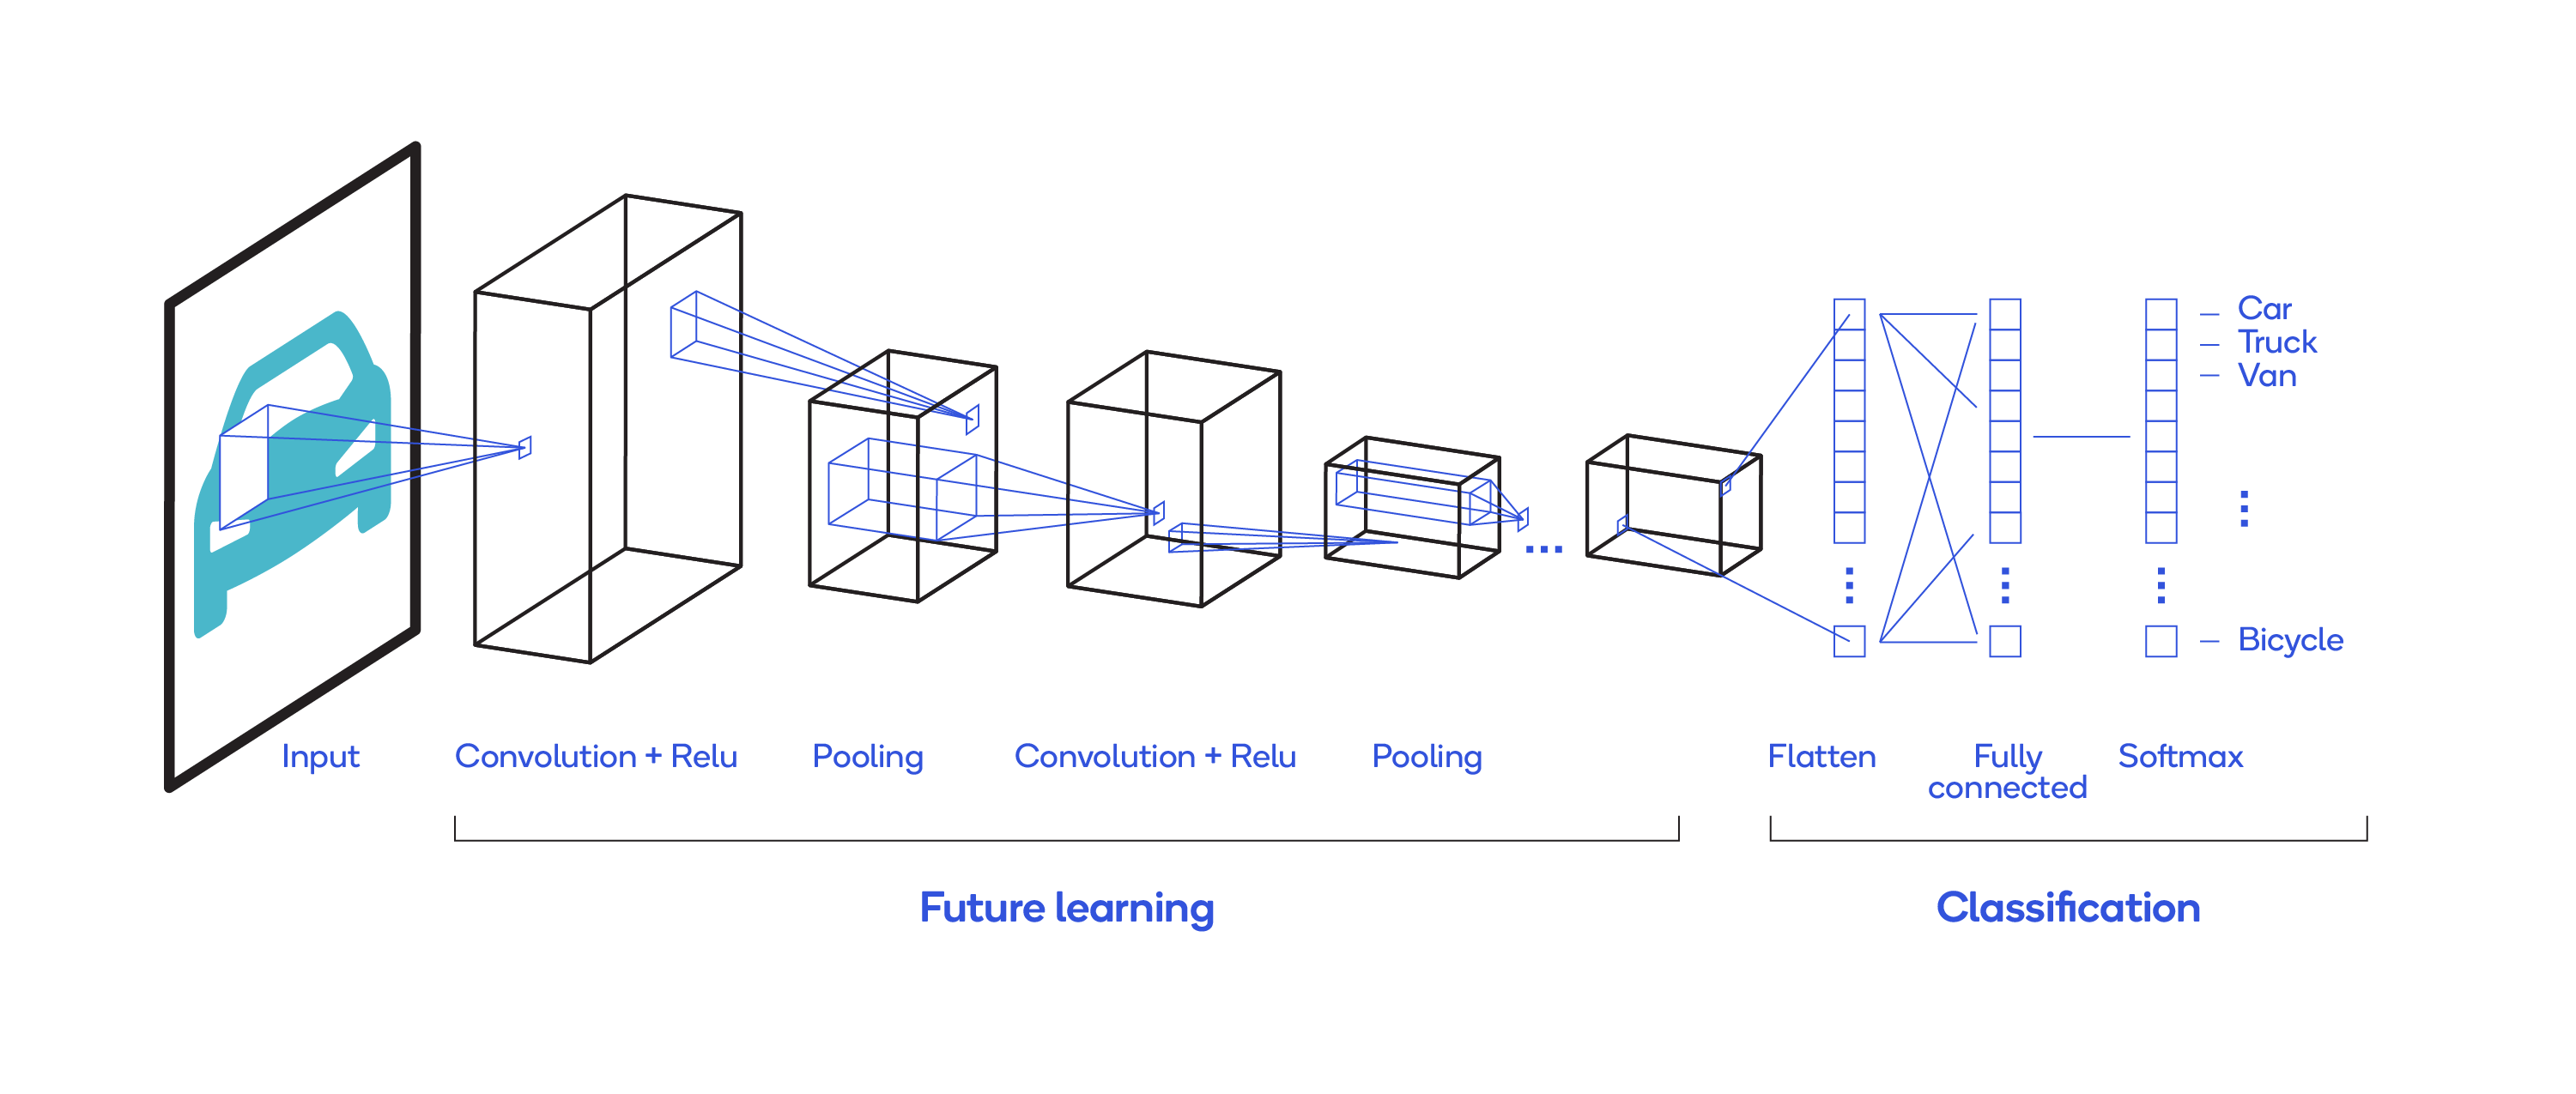
\includegraphics[width=\textwidth]{resources/images/CNN.png}
    \caption{A neural network architecture for image classification task, constructed from convolutional layer, pooling layer and fully-connected layer.}
    \label{fig:cnn}
\end{figure}
Concretely, a simple ConvNet is constructed from a sequence of individual layers (illustrated in figure \ref{fig:cnn}): \\
\textbf{Convolutional Layer}. \quad The most important component in a CNN architecture. Receive an input volume from previous layer, the layer apply a convolution function using an adaptive \textit{kernel} (or \textit{filter}) to compute outcome neurons for current layer. The operation works as sliding the \textit{kernel} across the entire input then compute dot product between the covered input values and the filter entries. An activation function is also applied on each neuron value, as mentioned in \ref{model:mlp}. By this function, we output a 2D feature map with the shape usually smaller than the input volume. Intuitively, the convolution works as a pattern identifier, aims to extract visual feature given in images such as object edges or other special shapes, etc. \\
Some important hyper-parameters used to define a convolutional layer:
\begin{itemize}
    \item Kernel size: $[K \times K \times C_{in}]$, predefined shape of filter matrix used in convolution process. $C_{in}$ is the input channel of input tensor from previous layer.
    \item Number of kernel: $N_{k}$, the amount of kernels we apply at the current layer. Each kernel correspondents to a specific convolution layer, used to produce a 2D feature map. Finally, we stack these maps to achieve the output volume.
    \item Stride: $S$, the number of pixels that the kernel splits on the tensor.
    \item Padding: $P$, the number of rows/columns used to pad the input around the border. This step helps to reduce the information loss as the border pixels are not used as frequently as the inner ones.    
\end{itemize}
\textbf{Pooling Layer}. \quad The layer used to reduce the spatial size of the output feature map produced by successive convolutional layer. This technique helps to reduce computation cost and amount of parameters, and hence, help to control overfitting. \\
\textbf{Fully-Connected Layer}. \quad The layer performs exactly as a Neural Network mentioned in section \ref{model:mlp}. Receive the final representation from previous step, fully-connected layer provides a stack of dense connection to get the final prediction for a specific task. For example in image classification problem, the layer produce an output vector $\mathbf{o} \in \mathbb{R}^{c}$ ($c$ is the number of target classes), then apply a softmax function to give prediction confidence. \\
% Figure ... shows an example of a typical CNN architecture.\\
In general, ConvNet can be seen as a two-stage process, feature learning and prediction. The feature learning stage built from stack of convolution-pooling blocks, aims to produce the final representation of the input image while the prediction stage utilizes this embedded information for a specific tasks.
Therefore, the ConvNet is also commonly used for feature extraction and can be efficiently applied in various tasks such as Image/Video Retrieval, Instance Re-identification or Image Generation, etc. 

% \subsection{Modern convolutional networks}
% In this section, we 
% [TODO]